\documentclass{article}

\usepackage{amsmath, amssymb, amsthm}
\usepackage[a4paper, margin=2.5cm]{geometry}
\usepackage{graphicx}
\usepackage{svg}
\usepackage{float}
\usepackage{caption}
\usepackage{hyperref}
\usepackage{parskip}
\usepackage{lipsum}

\title{Autograd in NumPy}
\author{Luke Zeng}
\date{}

\renewcommand{\bottomfraction}{0.85}
\renewcommand{\textfraction}{0.1}

\begin{document}

\maketitle

\section{Introduction}
In this article, we will implement a simple autograd system in NumPy from scratch. Autograd is a technique for automatically computing gradients of functions, which is essential for training machine learning models without manually deriving gradients. We will define a class for tensors that can track operations and compute gradients, as well as some basic operations like addition and matrix multiplication. We will also implement a simple ReLU activation function and demonstrate how to use our autograd system to compute gradients for a simple neural network.

\section{Autograd Implementation}
The fundamental data structure in our autograd system will be the \texttt{Tensor} class. This class stores data (in a NumPy array) and tracks the operation that created it.

We also define an \texttt{AutogradFunction} class that represents a differentiable operation. Each operation will have a forward pass that computes the output and a backward pass that computes the gradient with respect to its inputs using the chain rule.

Autograd works by building a computational graph during the forward pass, where each node represents an operation/function and edges represent the flow of data (tensors). During the backward pass, we traverse this graph in reverse (normally from the loss to the leaf nodes) to compute gradients.

Figure~\ref{fig:autograd_graph} illustrates a simple computational graph for a neural network. In order to traverse the graph during the backward pass, we can start from the output node (e.g., the loss) and recursively compute gradients for each node by applying the chain rule. For instance, the gradient of the loss with respect to the output of the last layer (the Add node) can be computed, and then we can use the chain rule to compute the gradients with respect to the inputs of the Add node (the output of the MatMul and the bias). This process continues until we reach the leaf nodes (inputs and parameters), at which point we will have computed the gradients needed for optimization.

\begin{figure}[b]
    \centering
    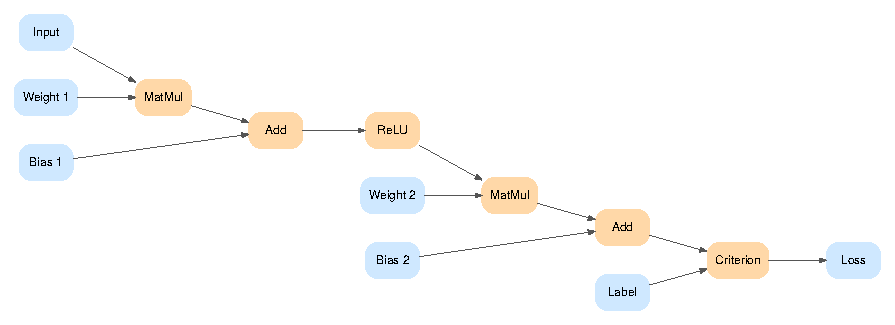
\includegraphics[width=0.62\textwidth]{assets/figure1_computational_graph}
    \captionsetup{width=0.62\textwidth}
    \caption{A simple computational graph for a neural network. The blue nodes represent leaf tensors (inputs and parameters) and outputs, while the orange nodes represent tensors that result from operations (e.g., matrix multiplication, addition, ReLU). The edges indicate the flow of data and gradients during the forward and backward passes. For example, since matrix multiplication is a binary operation, the node for the matrix multiplication will have two incoming edges.}
    \label{fig:autograd_graph}
\end{figure}

A simple case to consider is the scenario where every node represents a scalar value. In this case, we do not have to consider the complexities of computing the gradient of the loss function with respect to a tensor, but rather the partial derivative of the loss function with respect to a scalar. Figure~\ref{fig:scalar_computational_graph} illustrates a simple computational graph where every weight and input is a scalar (and thus every intermediate node is also a scalar).

In this case, the backward pass is straightforward, as we can directly apply the chain rule to compute the gradients for each node without worrying about the dimensions of tensors. For instance, we can start by defining:
\[
    \text{loss} = f(\text{output}, \text{label})
\]
where $f$ is a loss function (e.g., mean squared error). We can then compute the gradient of the loss with respect to the output as:
\[
    \frac{\partial \text{loss}}{\partial \text{output}} = \frac{\partial f}{\partial \text{output}}
\]

Then we can compute the gradient of the loss with respect to the multiplication node and the bias node as:
\[
    \frac{\partial \text{loss}}{\partial \text{mul}} = \frac{\partial \text{loss}}{\partial \text{output}} \cdot \frac{\partial \text{output}}{\partial \text{mul}}
\]
and the gradient with respect to the bias node as:
\[
    \frac{\partial \text{loss}}{\partial \text{bias}} = \frac{\partial \text{loss}}{\partial \text{output}} \cdot \frac{\partial \text{output}}{\partial \text{bias}}
\]

Since the output node is the result of an addition operation ($\text{output} = \text{mul} + \text{bias}$), we can compute the gradient with respect to the multiplication node and the bias node as:

\[
    \frac{\partial \text{output}}{\partial \text{mul}} = 1
, \quad
    \frac{\partial \text{output}}{\partial \text{bias}} = 1
\]

and thus we have:
\[
    \frac{\partial \text{loss}}{\partial \text{mul}} = \frac{\partial \text{loss}}{\partial \text{output}}
, \quad
    \frac{\partial \text{loss}}{\partial \text{bias}} = \frac{\partial \text{loss}}{\partial \text{output}}
\]

The bias node is a leaf node, so we can stop the backward pass there. For the multiplication node ($\text{mul} = \text{weight} \cdot \text{input}$), we can compute the gradient with respect to its inputs (the weight and the input) as:
\[
    \frac{\partial \text{loss}}{\partial \text{weight}} = \frac{\partial \text{loss}}{\partial \text{mul}} \cdot \frac{\partial \text{mul}}{\partial \text{weight}} = \frac{\partial \text{loss}}{\partial \text{mul}} \cdot \text{input}
    , \quad
    \frac{\partial \text{loss}}{\partial \text{input}} = \frac{\partial \text{loss}}{\partial \text{mul}} \cdot \frac{\partial \text{mul}}{\partial \text{input}} = \frac{\partial \text{loss}}{\partial \text{mul}} \cdot \text{weight}
\]

We can continue this process for any additional nodes in the computational graph, applying the chain rule at each step until we have computed the gradients for all leaf nodes. Then, we can use these gradients to perform optimization (e.g., using gradient descent) to update the parameters of our model.


\begin{figure}[b]
    \centering
    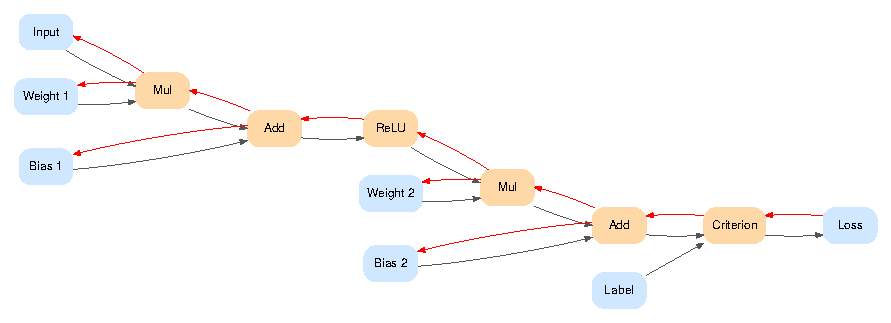
\includegraphics[width=0.62\textwidth]{assets/figure2_scalar_computational_graph}
    \captionsetup{width=0.62\textwidth}
    \caption{A simple computational graph where every weight and input is a scalar (and thus every intermediate node is also a scalar). The red edges indicate the flow of gradients during the backward pass.}
    \label{fig:scalar_computational_graph}
\end{figure}

The case where every node represents a scalar value is a special case of the more general scenario where nodes can represent tensors of arbitrary dimensions. In the general case, we need to consider the shapes of tensors and how to compute gradients with respect to them, which can involve more complex operations (e.g., matrix multiplication, broadcasting). However, the underlying principle of using the chain rule to compute gradients remains the same regardless of whether we are dealing with scalars or tensors.

\subsection{Functions and Operations}

We can define various functions and operations that our autograd system will support. Our implementation will include all the basic operations needed to build and train a simple neural network, such as addition, multiplication, matrix multiplication, ReLU, and a loss function (e.g., Cross-Entropy Loss). Each of these operations will have a corresponding backward function that computes the gradient with respect to its inputs.

\subsubsection{Matrix Multiplication}

\textbf{Forward.} Given inputs $X \in \mathbb{R}^{m \times k}$ and $W \in \mathbb{R}^{k \times n}$,
\[
    Z = XW, \quad Z \in \mathbb{R}^{m \times n}
\]

\textbf{Backward.} Let $\bar{Z} = \dfrac{\partial L}{\partial Z}$ be the upstream gradient. By the chain rule,
\begin{align}
    \frac{\partial L}{\partial X} &= \bar{Z}\, W^\top \\
    \frac{\partial L}{\partial W} &= X^\top \bar{Z}
\end{align}

\subsubsection{Addition}
\textbf{Forward.} Given inputs $A$ and $B$, 
\[
    C = A + B
\]
\textbf{Backward.} Let $\bar{C} = \dfrac{\partial L}{\partial C}$ be the upstream gradient. By the chain rule,

\begin{align}
    \frac{\partial L}{\partial A} &= \bar{C} \\
    \frac{\partial L}{\partial B} &= \bar{C}
\end{align}
\subsubsection{ReLU}
\textbf{Forward.} Given input $X$,
\[
    Y = \text{ReLU}(X) = \max(0, X)
\]
\textbf{Backward.} Let $\bar{Y} = \dfrac{\partial L}{\partial Y}$ be the upstream gradient. By the chain rule,
\[
    \frac{\partial L}{\partial X} = \bar{Y} \cdot \mathbf{1}_{X > 0}
\]
\subsubsection{Cross-Entropy Loss}
\textbf{Forward.} Given predicted probabilities $P$ and true labels $Y$ (one-hot encoded),
\[
    L = -\sum_{i} Y_i \log(P_i)
\]
\textbf{Backward.} Let $\bar{L} = \dfrac{\partial L}{\partial L} = 1$ be the upstream gradient. By the chain rule,
\[
    \frac{\partial L}{\partial P_i} = -\frac{Y_i}{P_i}
\]

\subsubsection{Softmax}
\textbf{Forward.} Given input $Z$,
\[
    P_i = \frac{e^{Z_i}}{\sum_j e^{Z_j}}
\]
\textbf{Backward.} Let $\bar{P} = \dfrac{\partial L}{\partial P}$ be the upstream gradient. By the chain rule,
\[
    \frac{\partial L}{\partial Z_i} = \sum_j \frac{\partial L}{\partial P_j} \cdot \frac{\partial P_j}{\partial Z_i}
\]

Note that in practice, we often combine the softmax function with the cross-entropy loss for numerical stability, which leads to a simplified backward pass.

Now that we have defined the forward and backward passes for our operations, we can implement the \texttt{Tensor} class to track these operations and compute gradients automatically. The \texttt{Tensor} class will store the data, the gradient, and a reference to the function that created it (if any). During the backward pass, we will recursively call the backward functions of each operation in the computational graph to compute gradients for all tensors.


% \lipsum[1-2]

\end{document}

